% !TeX encoding = ISO-8859-1
% Resources 
\chapter{Recursos}

% Personnel 
\section{Pessoal}

% Size of staff for the project 
\subsection{Tamanho da equipe para o projeto }

Caroline Correa, Marco Aurélio Souza, Rafael Santos

% Software 
\section{Software}

% Identify  software  needed  to  support  system  (includes  system  plus SEE/STE/tools requirements) 
\subsection{Identificar o software necessário para suportar o sistema}

JDK 8, MySQL, Netbeans, Git

% Hardware 
\section{Hardware}

% Identify hardware needed to support system (includes system plus SEE/STE requirements) 
\subsection{Identificar o hardware necessário para suportar o sistema}

Notebook com 4gb de RAM

% Facilities 
\section{Instalações}

% Identify facilities requirements
\subsection{Identificar requisitos de instalações}

Acesso à internet

% Special procedural requirements (e.g., security, access rights, and documentation control)
\section{Requisitos processuais especiais (por exemplo, segurança, direitos de acesso e documentação ao controle)}

\pagebreak

% Cost estimating 
\section{Estimativa de custo}

\begin{figure}[ht]
	\centering
	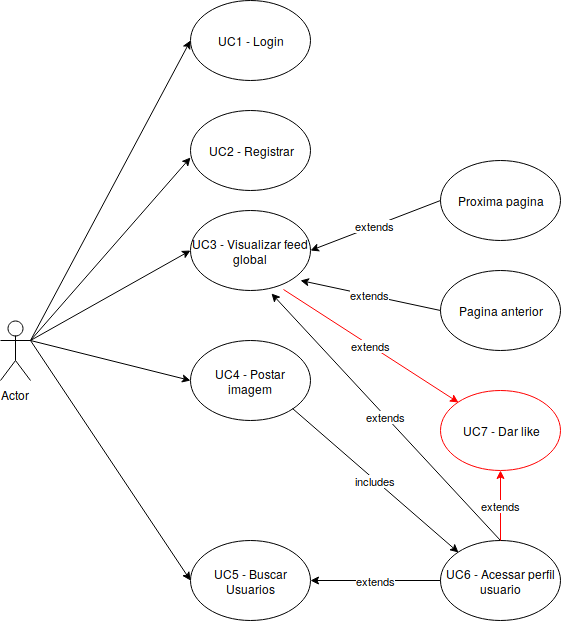
\includegraphics[width=\textwidth]{./g/casodeuso.png}
	\caption{Diagrama de caso de uso}
	\label{fig:casoDeUso}
\end{figure}

\begin{table}[!htb]
	\caption[Atores]{Relação de atores e seus respectivos pesos}
	\label{tab:correlacao}
	\centering
	\begin{tabular}{c|c}
		Atores  & Peso 	\\ \hline
		Cliente & 3    	\\
		Site    & 2		\\
	\end{tabular}
\end{table}

\begin{table}[!htb]
	\caption[TPNAA]{Total de Pesos não ajustados dos Atores}
	\label{tab:correlacao}
	\centering
	\begin{tabular}{c|c|c|c}
		Complexidade 		 & Qtde. Atores 			& Peso 		 & Resultado	\\ \hline
		1 					 & 0						&	1		 &	  0 	 	\\
		2 					 & 1						&	2		 &	  2 	 	\\
		3 					 & 1						&	3		 &	  3 	 	\\ \hline
		\multicolumn{4}{l}{Total de Pesos não Ajustados dos Atores(TPNAA) = 5}	 	\\
	\end{tabular}
\end{table}

\begin{table}[!htb]
	\caption[Atores]{Relação Casos de Uso}
	\label{tab:correlacao}
	\centering
	\begin{tabular}{c|c}
		Casos de Uso 		& Peso  \\ \hline
		Login       		& 3     \\
		Registrar    		& 1     \\
		Visualizar Feed	& 3     \\
		Postar Imagem		& 3     \\
		Acessar Perfil	& 2     \\
		Dar Like				& 3     \\
		Fazer Comentário	& 2     \\
	\end{tabular}
\end{table}


\begin{table}[!htb]
	\caption[TPNACU]{Total de Pesos não ajustados dos Casos de Uso}
	\label{tab:correlacao}
	\centering
	\begin{tabular}{c|c|c|c}
		Complexidade & Qtde. Casos de Uso & Peso & Resultado	\\ \hline
		1 			 &  		1		  &	1	 &	  1 		\\
		2 			 &  		2		  &	2	 &	  4 		\\
		3 			 &  		4		  &	3	 &	  12 		\\ \hline
		\multicolumn{4}{l}{Total de Pesos não ajustados dos Casos de Uso(TPNACU) = 17} \\
	\end{tabular}
\end{table}

PTNA = TPNAA + TPNACU
PTNA = 5 + 17
PTNA = 22

\begin{table}[!htb]
\caption[FCA]{Fator de Complexidade Ambiental}
	\label{tab:correlacao}
	\centering
	\begin{tabular}{c|c|c|c|c}
		Fator & Descricao										                    & Peso	& Valor & EFator   \\   \hline
		F1	  & Familiaridade com Processo Iterativo Unificado	& 1.5	  &	 4    &		6		\\
		F2	  & Experiencia na Aplicação						            & 0.5	  &	 4    &		2 	 	\\
		F3 	  & Experiência em orientação a objetos				      & 1		  &  4    &		4 		\\
		F4 	  & Capacidade de Liderança de Análise				      & 0.5	  &	 3    &		1.5 		\\
		F5 	  & Motivação										                    & 1		  &	 1    &		1 		\\
		F6 	  & Estabilidade dos Requisitos						          & 2		  &  4    &		8 		\\
		F7 	  & Consultores Part-Time							              & -1	  &	 0    &		0 		\\
		F8 	  & Dificuldade de Programação na Linguagem			    & -1	  &	 2    &		-2 		\\ \hline
		\multicolumn{5}{l}{Total(EFator) = ?}\\ \hline
		\multicolumn{5}{l}{FCA => 1.4 + (-0.03 * 20.5) = 0.785}\\
	\end{tabular}
\end{table}


\begin{table}[!htb]
\caption[FCT]{Fator de Complexidade Técnica}
	\label{tab:correlacao}
	\centering
	\begin{tabular}{c|c|c|c|c}
		Fator & Descricao								   & Peso & Valor &     \\ \hline
		T1	  & Distribuição do sistema 				  				 & 2 	  &	  5   &	  10	  \\
		T2	  & Respostas aos objetivos de desempenho      & 1 	  &	  3   &	 	3  \\
		T3 	  & Eficiência do usuário final                & 1 	  &	  3   &		3	  \\
		T4 	  & Complexidade do Processo Interno           & 1 	  &	  5   &		5	  \\
		T5 	  & Código deve ser reutilizado                & 1 	  &	  4   &		4	  \\
		T6 	  & Facilidade de instalação                   & 0.5  &	  5   &		2.5	  \\
		T7 	  & Facilidade de uso                          & 0.5  &	  5   &		2.5	  \\
		T8 	  & Portabilidade                              & 2	  &	  4   &		8	  \\
		T9 	  & Facilidade de alterar                      & 1	  &	  2   &		2	  \\
		T10	  & Concorrência                               & 1	  &	  4   &		4	  \\
		T11	  & Features de segurança                      & 1	  &	  2   &		2	  \\
		T12	  & Acesso direto a dispositivos parceiros     & 1	  &	  0   &		0	  \\
		T13	  & Treinamento especial aos usuários          & 1	  &	  0   &		0	   \\ \hline
		\multicolumn{5}{l}{Total(TFator) = 46}\\ \hline
		\multicolumn{5}{l}{FCT => 0.6 + (0.01 * 46) = 1.06}\\
	\end{tabular}
\end{table}

PTUC = PTNA * FCT* FCA

PTUC = 22 * 0.785 * 1.06

PTUC = 18.3

Estimativas com os pontos obtidos

Sugestão de Karner = PTUC * 20

Sugestão de Karner = 18.3 * 5 = 91.5 horas

91.5 horas / (3 horas por dia * 2 pessoas) = 15.25 dias

15.25 dias / 5 dias por semana =  3 semanas

91.5 horas *  75 reais por hora = R\$ 6862,50 total manutenção

Preço da hora
% Describe the cost estimating method 
\subsection{Método da estimativa de custo}

Pontos por caso de uso

% Documentation 
\section{Documentação}

% Software Quality Plan
\subsection{Plano de qualidade do software}
	Será feito uma avaliação das modificações implementadas segundo as normas da ISO 9126.
% Project Management Plan 
\subsection{Plano de Gerenciamento de Projeto}

Trello

% Configuration Management Plan
\subsection{Plano de Gerenciamento de Configuração}

GitHub

% Measurement Plan
\subsection{Plano de Medição}

% Development documents
\subsection{Documentos de desenvolvimento}

\subsubsection{Diagrama de Caso de Uso}

\begin{figure}[ht]
	\centering
	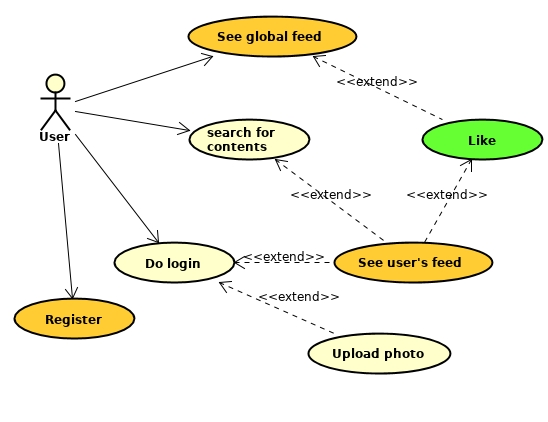
\includegraphics[width=\textwidth]{./imagens/usecase.png}
	\caption{Diagrama de caso de uso}
	\label{fig:casoDeUso}
\end{figure}

\subsubsection{Diagrama de Classes}
\begin{figure}[ht]
	\centering
	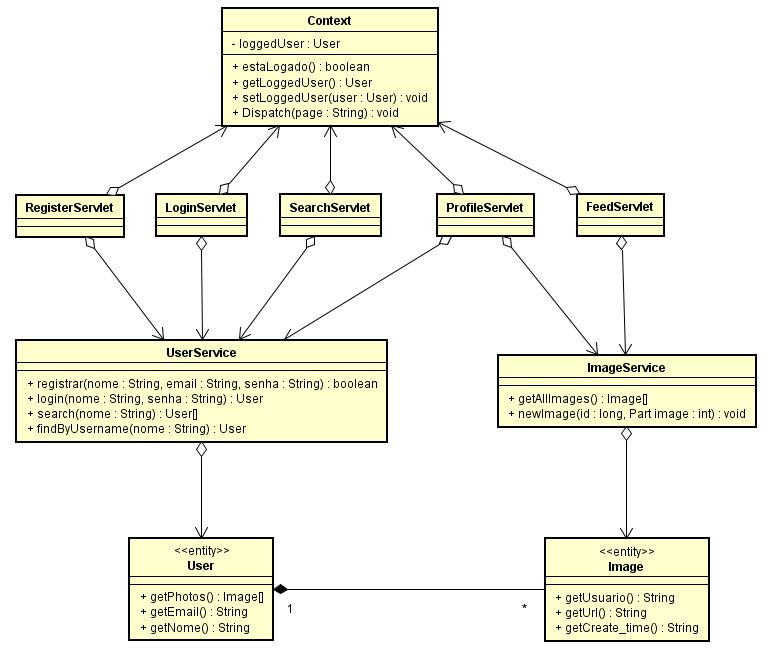
\includegraphics[width=\textwidth]{./imagens/classdiagram.png}
	\caption{Diagrama de classes}
	\label{fig:diagramaDeClasse}
\end{figure}

\subsubsection{Modelo Relacional} 
\begin{figure}[ht]
	\centering
	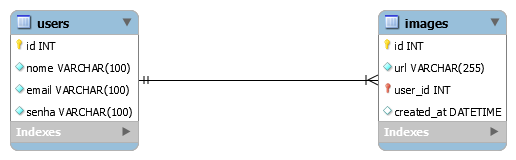
\includegraphics[width=\textwidth]{./imagens/der.png}
	\caption{Modelo Relacional}
	\label{fig:modeloRelacional}
\end{figure}

% Maintenance manuals
\subsection{Manuais de manutenção}

% Verification Plan
\subsection{Plano de Verificação}

% Validation Plan
\subsection{Plano de validação}

% Test Plan, Test Procedures, and Test Reports
\subsection{Plano de teste, procedimentos de teste e relatórios de teste}

\subsubsection{Plano de teste}

Teste Funcional Caixa Preta.

\subsubsection{Procedimentos}

Utilizar o software manualmente.

\subsubsection{Relatórios de Teste}
O teste foi feito manualmente no software, e em cada erro encontrado, definiu-se as correções e as melhorias para a manutenção do mesmo.

% Training Plan 
\subsection{Plano de Treinamento}

 Será apresentado ao usuário uma lista de modificações com prints das telas de antes e depois da manutenção. 
 As telas serão mostradas como um storyboard do sistema de acordo com as manutenções.

% User?s Manual(s)
\subsection{Manual(s) do Usuário}
Antes
\subsubsection{Formulário sem o campo confirmar senha}
\begin{figure}[ht]
	\centering
	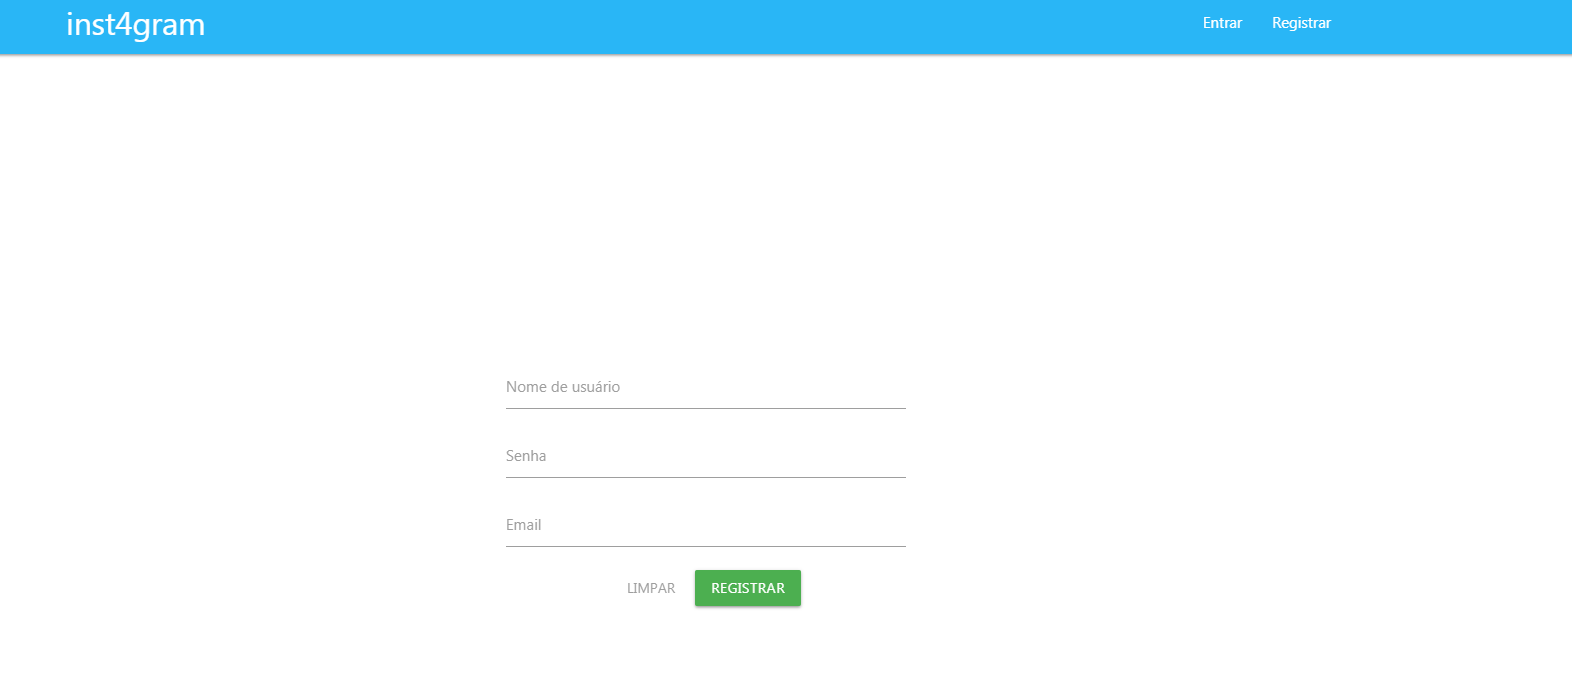
\includegraphics[width=0.5\textwidth]{./imagens/confirmacao_senha.png}
	\caption{Diagrama de caso de uso}
	\label{fig:casoDeUso}
\end{figure}

\pagebreak

\subsubsection{Mostrando páginas vazias}
\begin{figure}[ht]
	\centering
	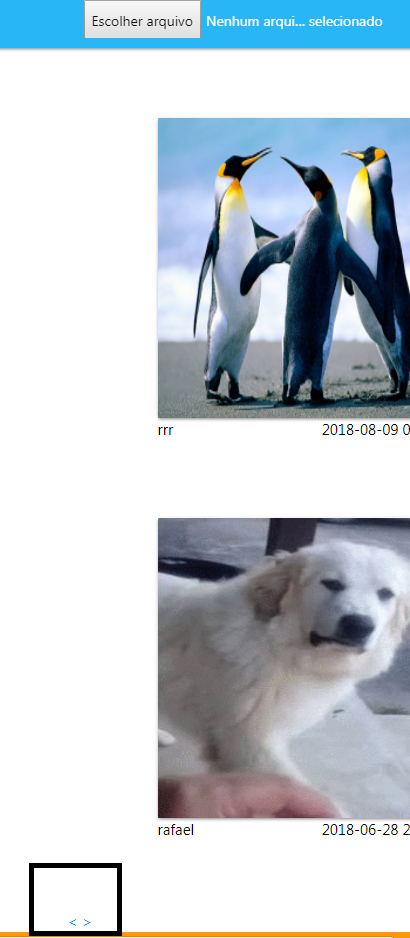
\includegraphics[width=0.5\textwidth]{./imagens/paginas.png}
	\caption{Diagrama de caso de uso}
	\label{fig:casoDeUso}
\end{figure}

\pagebreak

\subsubsection{Página sem a funcionalidade de curtir a imagem}
\begin{figure}[ht]
	\centering
	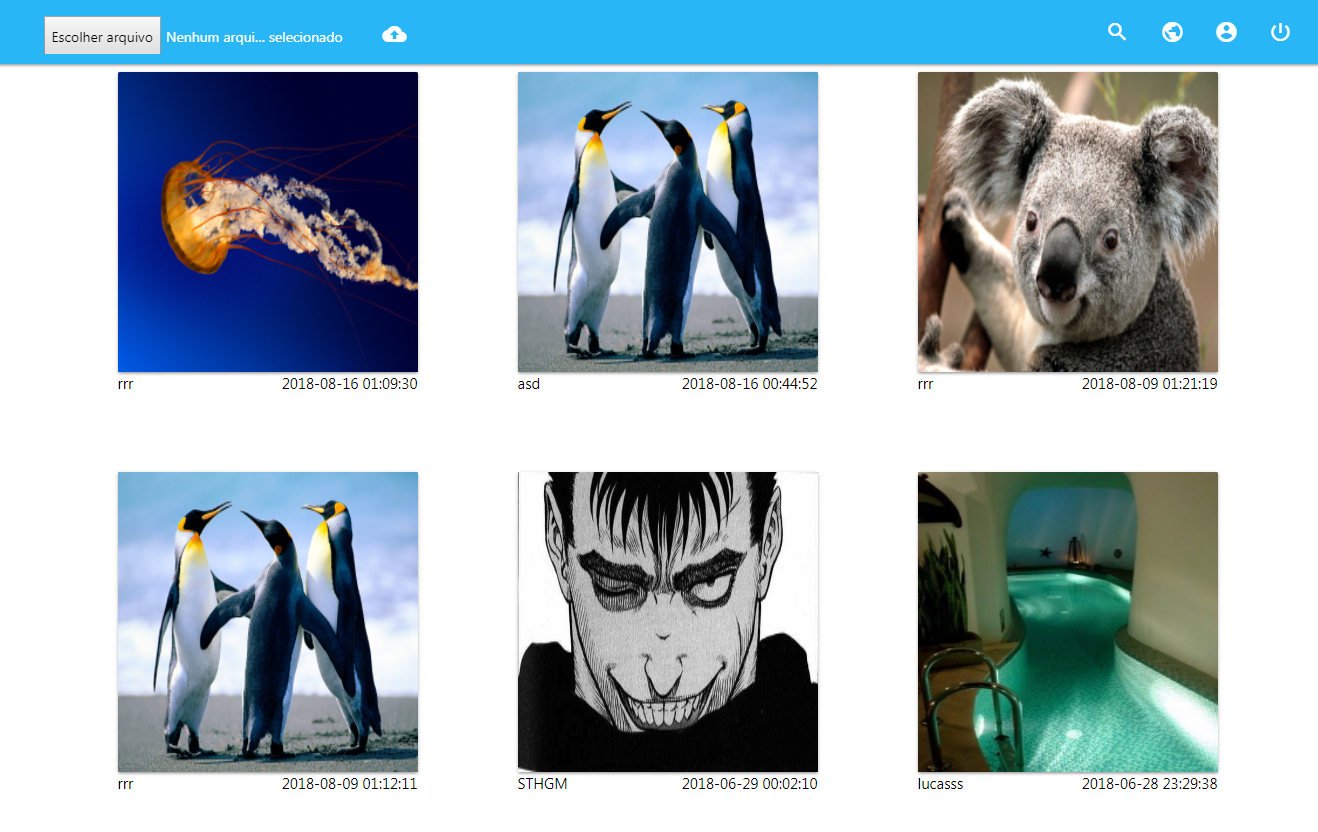
\includegraphics[width=0.5\textwidth]{./imagens/botao_curtir.png}
	\caption{Diagrama de caso de uso}
	\label{fig:casoDeUso}
\end{figure}

\pagebreak

\subsubsection{Perfil incompleto}
\begin{figure}[ht]
	\centering
	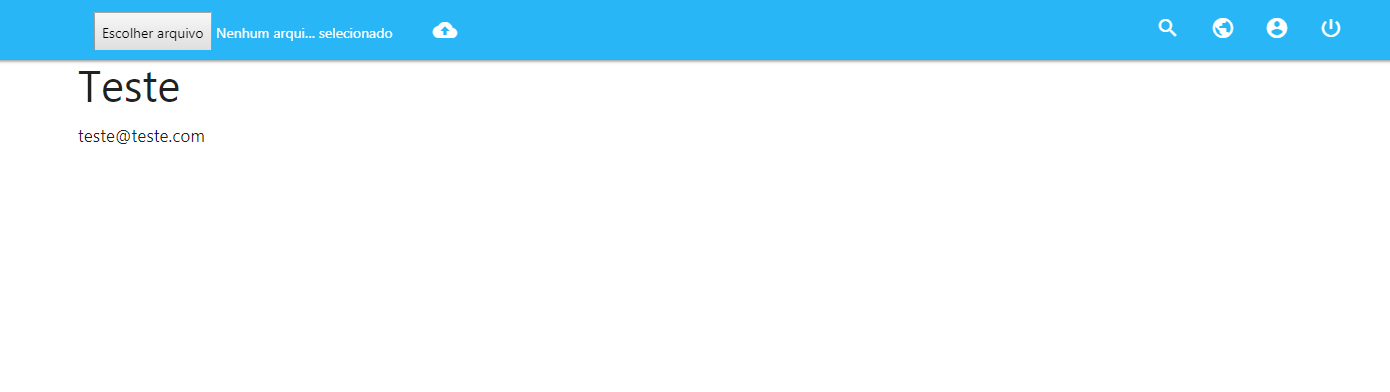
\includegraphics[width=0.5\textwidth]{./imagens/perfil_desarrumado.png}
	\caption{Diagrama de caso de uso}
	\label{fig:casoDeUso}
\end{figure}

\pagebreak

\subsubsection{Permitindo o envio de qualquer tipo de arquivo diferente de uma imagem}
\begin{figure}[ht]
	\centering
	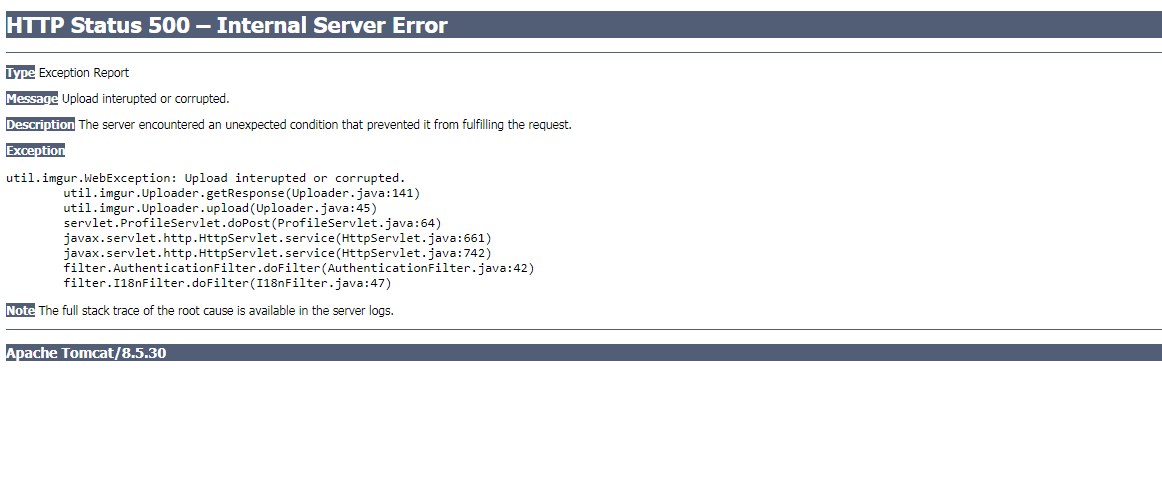
\includegraphics[width=0.5\textwidth]{./imagens/erro_envio.png}
	\caption{Diagrama de caso de uso}
	\label{fig:casoDeUso}
\end{figure}

\pagebreak

\subsubsection{Correção de botão}
\begin{figure}[ht]
	\centering
	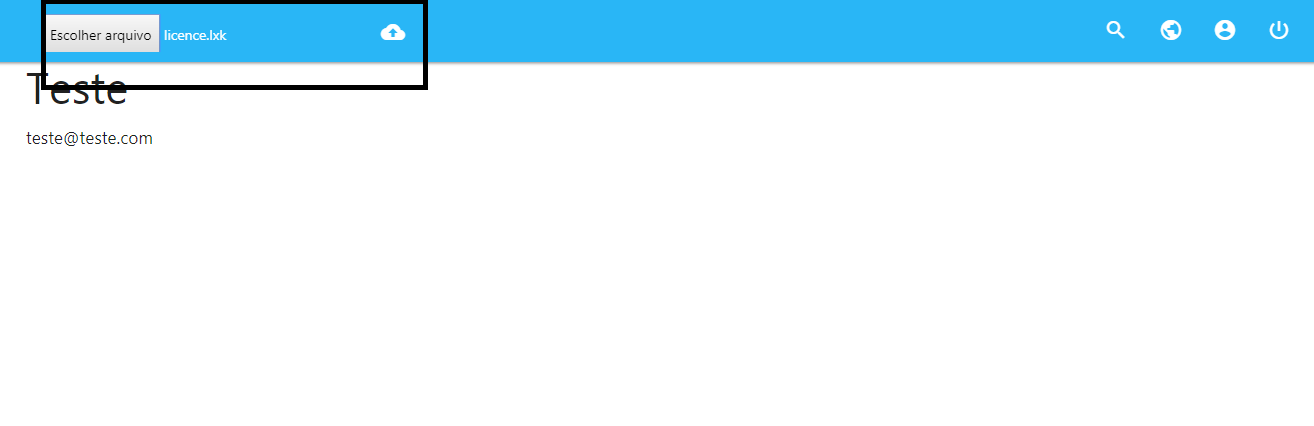
\includegraphics[width=0.5\textwidth]{./imagens/envio_qualquer_arquivo.png}
	\caption{Diagrama de caso de uso}
	\label{fig:casoDeUso}
\end{figure}

\pagebreak


\subsubsection{Sem nome de usuário na tela principal}
\begin{figure}[ht]
	\centering
	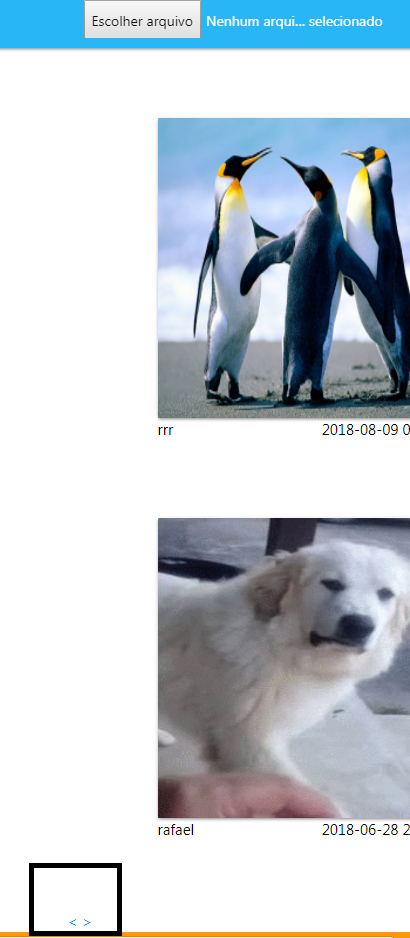
\includegraphics[width=0.5\textwidth]{./imagens/paginas.png}
	\caption{Diagrama de caso de uso}
	\label{fig:casoDeUso}
\end{figure}

\pagebreak

Depois


% Data management
\section{Gerenciamento de dados}

% Identify repositories 
\subsection{Repositórios}
Documento
https://github.com/rafaelnsantos/manutencao-software

Software
https://github.com/web-2-utfpr/instaclone

% Other resource requirements (if needed)
\section{Outros requisitos de recursos (se necessário)}
